\documentclass[fr]{../../../eplsummary}

\usepackage{../../../eplunits}
\usepackage{../../../eplelec}
\usepackage{circuitikz}
\sisetup{detect-all}

\makeatletter
\providecommand\add@text{}
\renewcommand\u[1]{%
  \gdef\add@text{[\si{#1}\gdef\add@text{}]}}% 
\renewcommand\tagform@[1]{%
  \maketag@@@{\llap{\add@text\quad}(\ignorespaces#1\unskip\@@italiccorr)}%
}
\makeatother

\hypertitle{\'{E}lectromagnétisme appliqué}{5}{ELEC}{1350}
{Antoine Paris}
{Christophe Craeye et Danielle Janvier}

\section{Loi de Coulomb et champ électrique}
\subsection{Loi de Coulomb}
\begin{mylaw}
La loi de Coulomb est une loi expérimentale qui
décrit la force d'attraction (ou de répulsion)
entre deux charges
\begin{equation}
	\vec{F} = \frac{q_1q_2}{4\pi\perm_0r^2}\hat{a}_r
	\u{\newton}
\end{equation}

Cette force agit sur la ligne joignant les deux charges
et est répulsive si les charges sont
de même signe, attractive dans le cas contraire.
\end{mylaw}

\subsection{Champ électrique}
\begin{mydef}
Le champ électrique subi par une charge $q$
est défini comme la force électrique subie
par unité de charge
\begin{equation}
	\E \eqdef \frac{\vec{F}}{q}.
	\u{\newton\per\coulomb}
	\label{eq:electric-field}
\end{equation}
\end{mydef}

\subsubsection{D'une seule charge}
\begin{equation}
	\E = \frac{q}{4\pi\perm_0r^2}\hat{a}_r
\end{equation}

\begin{myprop}
Le champ électrique étant une fonction linéaire
de la charge, le principe de superposition s'
applique.
\end{myprop}

\subsubsection{D'une distribution de charge}
Pour une distribution de charge (linéique, de surface
ou de volume), on a
\begin{equation}
	Q = \int_{\text{vol}} \rho_v\dif v
	\u{\coulomb}
\end{equation}

En définissant un référentiel quelconque comme
sur la figure \ref{fig:referentiel}, on peut
écrire $\vec{E}$ de manière tout à fait générale
\begin{equation}
	\vec{E}(r) = \int_{\text{vol}} \frac{\rho_v(r')\dif v}{4\pi\perm_0|r-r'|^2}
	\frac{r - r'}{|r - r'|}
\end{equation}

\begin{figure}
	\centering
	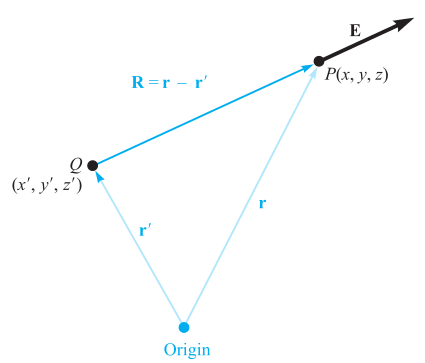
\includegraphics[scale=0.5]{img/referentiel.png}
	\caption{Référentiel quelconque.}
	\label{fig:referentiel}
\end{figure}

\section{Densité de flux électrique, loi de Gauss et divergence}
\subsection{Champ de déplacement électrique}
Le champ de déplacement électrique ou densité de flux
électrique est donné par
\begin{equation}
	\D = \perm \E
	\u{\coulomb\per\meter\squared}
\end{equation}

\subsection{Loi de Gauss}
\begin{mylaw}
Le flux électrique à travers une surface
fermée est égal à la quantité de charge située à
l'intérieur de cette surface fermée.
\end{mylaw}

Mathématiquement,
\begin{equation}
	\oint_\text{S} \vec{D}_\text{S} \cdot \dif \vec{S} 
	= \int_\text{vol} \rho_v \dif v = Q
	\label{eq:gauss}
\end{equation}

où $\vec{S}$ est défini comme sortant de la surface. 

La loi de Gauss permet de calculer des champs électriques
pour des distribubtions de charges symétriques.

On peut aussi écrire cette équation sous la forme
\begin{equation}
	\divn \D = \rho_v
\end{equation}

en se rappellant de la définition de la divergence.

\begin{mydef}
La divergence d'un vecteur de densité de
flux est égal au flux sortant d'une petit surface
fermée par unité de volume lorsque ce volume tend
vers zéro.
\end{mydef}

Une divergence positive indique donc la présence d'une
\textit{source} tandis qu'une divergence négative indique
la présence d'un \textit{puits}.

On peut passer d'une équation à l'autre en utilisant
le théorème de la divergence
\begin{equation}
	\oint_\text{S} \vec{D}_\text{S} \cdot \dif \vec{S}
	= \int_\text{vol} \divn \D \dif v
\end{equation}

\section{\'{E}nergie et potentiel}
\subsection{Potentiel}
Supposons que l'on veuille déplacer une charge $Q$ d'une
distance $\dif \vec{l}$ dans un champ électrique $\E$.
Par \ref{eq:electric-field}, la force sur cette charge
est
\[ \vec{F}_E = Q\E. \]

La composante de cette force dans la direction
$\dif \vec{l}$ est donc
\[ \vec{F}_{EL} = \vec{F}_E \cdot \hat{a}_l = Q\E\cdot \hat{a}_l. \]

Pour vaincre cette force et déplacer la charge, il
faut appliquer une force
\[ \vec{F}_{appl} = -Q\E \cdot \hat{a}_l. \]

Le travail effectué par une source externe pour
déplacer cette charge d'une distance $\dif l$ est
donc
\[ \dif W = -Q\E \cdot \hat{a}_l \dif l = -Q\E \cdot \dif \vec{l} \]

et le travail total pour déplacer une charge d'un
point $A$ à un point $B$ est donné par
\[ W = -Q \int_A^B \E \cdot \dif \vec{l}. \]

\begin{mydef}
On définit ensuite la \textit{différence de potentiel} $V$
comme le travail effectué (par une source externe) pour
déplacer une charge unitaire positive d'un point à un
autre dans un champ électrique
\begin{equation}
	\Delta V = V_B - V_A = -\int_A^B \E \cdot \dif \vec{l}
	\u{\volt}
\end{equation}
\end{mydef}

Lorsqu'on utilise cette équation, on est souvent amené
à définir une référence de potentiel nul. En général, on
utilise pour cela soit un point de référence représentant
la \textit{terre} soit un point situé à une distance
\textit{infinie} du problème.

\begin{mydef}
Une \textit{surface équipotentielle} est une surface
composée de tous les points ayant le même potentiel.
Toutes les lignes de champ électrique sont perpendiculaires
à cette surface aux points d'intersections. Aucun travail
n'est donc nécessaire pour déplacer une charge sur une
surface équipotentielle.
\end{mydef}

\begin{myprop}
Aucun travail n'est effectué pour déplacer une charge
le long d'un chemin fermé
\begin{equation}
	\oint \E \cdot \dif l = 0.
	\label{eq:E-conservatif}
\end{equation}
Cette équation est valide pour les champs \textit{statique}.
On dit dans ce cas que $\E$ est un champ \textit{conservatif}.
On peut réecrire cette équation comme ceci
\begin{equation}
	\rotn \E = 0
\end{equation}
en utilisant les théorèmes intégraux.
\end{myprop}

Par conséquent, le champ $\E$ dérive d'un potentiel
\begin{equation}
	\E = - \gradn V.
\end{equation}
Cette équation nous permet d'obtenir un peu d'intuition
sur le champ électrique :
\begin{enumerate}
	\item La norme du champ électrique est donnée par la
	valeur maximum de la dérive du potentiel par à la
	distance ;
	\item La direction du champ électrique est opposée
	à la direction dans laquelle le potentiel augmente
	le plus rapidement.
\end{enumerate}

\subsection{Dipôle électrique}
\begin{mydef}
Un dipôle électrique est composé de deux charges ponctuelles
de normes égales mais de signe opposé séparé par une distance
faible par rapport à la distance à laquelle on veut calculer
le champ électrique.
\end{mydef}

\begin{mydef}
On définit le moment du dipole
\begin{equation}
	\vec{p} = Q\vec{d}.
\end{equation}
\end{mydef}

\subsection{Dénsité d'énergie}
\begin{equation}
	W_E = \frac{1}{2} \int_{vol} \D \cdot \E \dif v
	= \frac{1}{2} \int_{vol} \perm_0\E^2 \dif v
\end{equation}

\appendix

\section{Conducteurs et diélectriques}
\subsection{Conducteur électrique parfait et conditions limites}
\begin{myprop}
Un conducteur électrique parfait possède les propriétés
suivantes :
\begin{enumerate}
	\item La densité de charge à l'intérieur du conducteur
	est nulle ;
	\item Toutes les charges se trouvent sur la surface du
	conducteur.
\end{enumerate}
En électrostatique (pas de courant), on a en plus
\begin{enumerate}
	\item Le champ électrique à l'intérieur du conducteur
	est nul ;
	\item Le champ tangentiel à la surface est nul.
\end{enumerate}
\end{myprop}

Mathématiquement, en appliquant \ref{eq:E-conservatif} sur
le chemin rectangulaire de la figure \ref{fig:conductor-boundary},
on trouve bien que la composante tangentielle de $\E$ est nulle
\begin{equation}
	\E \times \hat{n} \Big|_s = 0.
\end{equation}
En appliquant \ref{eq:gauss} sur le cylindre de
la figure \ref{fig:conductor-boundary}, on trouve une
relation entre la composante normale à la surface et
la densité de charge du conducteur
\begin{equation}
	\D \cdot \hat{n} \Big|_s = \rho_s
\end{equation}
Dans ces deux équations, $\hat{n}$ est le vecteur unitaire
normal au conducteur et \textbf{sortant} du conducteur.

\begin{figure}[ht]
	\centering
	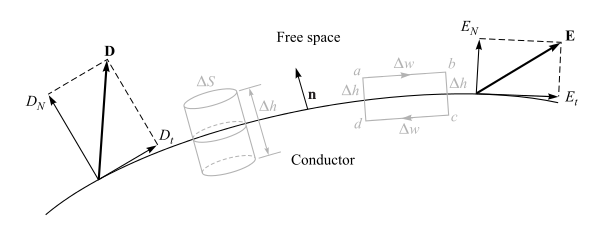
\includegraphics[scale=0.6]{img/conductor-boundary.png}
	\caption{Conditions limites pour un conducteur parfait.}
	\label{fig:conductor-boundary}
\end{figure}

\subsection{Diélectrique parfait et conditions limites}
En appliquant \ref{eq:E-conservatif} sur le chemin rectangulaire
de la figure \ref{fig:dielectric-boundary}, on trouve que le
le champ $\E$ tangentiel est continu aux interfaces
\begin{equation}
	(\E_1 - \E_2) \times \hat{n} = 0
\end{equation}
et donc automatiquement que le champ $\D$ tangentiel est
discontinu aux interfaces.

En appliquant \ref{eq:gauss} sur le cylindre de
la figure \ref{fig:dielectric-boundary}, on trouve
\begin{equation}
	(\D_1 - \D_2) \cdot \hat{n} = \rho_s
\end{equation}
où $\rho_s$ est la quantité de charge libre sur l'interface
(très souvent 0).

\begin{figure}[ht]
	\centering
	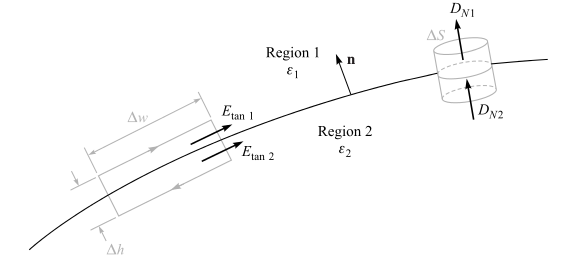
\includegraphics[scale=0.6]{img/dielectric-boundary.png}
	\caption{Conditions limites pour un diélectrique parfait.}
	\label{fig:dielectric-boundary}
\end{figure}

\section{Analyse vectorielle}

\begin{equation}
	\divn = \fpart{}{x}\vec{a}_x + \fpart{}{y}\vec{a}_y 
	+ \fpart{}{z}\vec{a}_z 
\end{equation}

\end{document}
